\documentclass{IEEEtran}

\usepackage{iansnotes}

\title{Graph Isomorphism}
\author{Ian McLoughlin}
\date{April 2021}
\setlength{\columnseprule}{0.4pt}
\begin{document}

\maketitle

\begin{description}[\setlabelwidth{$\alpha \omega \pi \theta \mu \mu$} \usemathlabelsep]
\item[$\gamma\delta\beta$] Is the index of..
\item[$\alpha\omega\pi\theta\mu$] Gives the..

\end{description}

 
    \section{Bijection}

  Map \( f \) from a set \( X \) to a set \( Y \) where:
  \begin{itemize}
    \item every \( y \) in \( Y \) is a value \( f(x) \) for at most one \( x \) in \( X \).
    \item every \( y \) in \( Y \) is a value \( f(x) \) for at least one \( x \) in \( X \).
  \end{itemize}
  \vspace{6mm}
  \begin{center}
    \begin{tikzpicture}
      \begin{scope}[every node/.style={circle, fill=black, inner sep=1pt}]
        \node[label=left:\( a \)] (a1) at (0,4) {};    
        \node[label=left:\( b \)] (a2) at (0,3) {};    
        \node[label=left:\( c \)] (a3) at (0,2) {};
        \node[label=left:\( d \)] (a4) at (0,1) {};
      
        \node[label=right:\( 1 \)] (b1) at (4,4) {};
        \node[label=right:\( 2 \)] (b2) at (4,3) {};
        \node[label=right:\( 3 \)] (b3) at (4,2) {};
        \node[label=right:\( 4 \)] (b4) at (4,1) {};
      \end{scope}
      
      \begin{scope}[every fit/.style={ellipse, draw,  inner sep=-2pt}]
        \node[draw, fit= (a1) (a2) (a3) (a4), minimum width=20mm] {} ;
        \node[draw, fit= (b1) (b2) (b3) (b4), minimum width=20mm] {} ;
      \end{scope}
      
      \path[->, >=latex, shorten <=2pt, shorten >=2pt] (a1) edge node[above] {\( f \)} (b1)
                                                       (a2) edge node[above] {\( f \)} (b2)
                                                       (a3) edge node[above] {\( f \)} (b3)
                                                       (a4) edge node[above] {\( f \)} (b4);  
    \end{tikzpicture} 
  \end{center}
  

  
\section{Isomorphism}

Two graphs \( G_1 = (V_1,E_1) \) and \( G_2=(V_2,E_2) \) are isomorphic, $G_1 \cong G_2$, when there is a bijection \( f \) from \( V_1 \) to \( V_2 \) such that \( \{f(x), f(y) \} \) is in \( E_2 \) if and only if \( (x,y) \) is in \( E_1 \).

\vspace{8mm}

  \begin{adjustbox}{max width={\columnwidth}, center}
    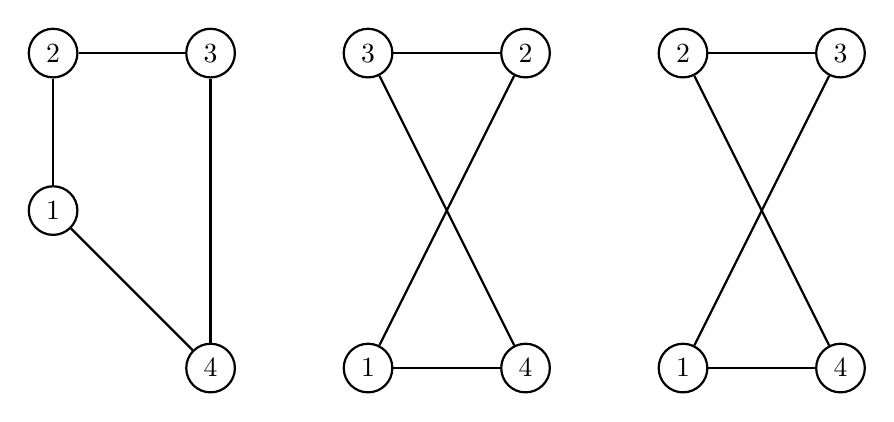
\begin{tikzpicture}
      \begin{scope}
        \begin{scope}[every node/.style={circle,thick,draw}]
          \node (a) at (0,2) {\( 1 \)};
          \node (b) at (0,4) {\( 2 \)};
          \node (c) at (2,4) {\( 3 \)};
          \node (d) at (2,0) {\( 4 \)};
        \end{scope}
        \begin{scope}[every edge/.style={draw=black,thick}]
          \path (a) edge (b)
                (b) edge (c)
                (c) edge (d)
                (d) edge (a);
        \end{scope}
      \end{scope}
      \begin{scope}[xshift=40mm]
        \begin{scope}[every node/.style={circle,thick,draw}]
          \node (a) at (0,0) {\( 1 \)};
          \node (c) at (0,4) {\( 3 \)};
          \node (b) at (2,4) {\( 2 \)};
          \node (d) at (2,0) {\( 4 \)};
        \end{scope}
        \begin{scope}[every edge/.style={draw=black,thick}]
          \path (b) edge (c)
                (c) edge (d)
                (b) edge (a)
                (d) edge (a);
        \end{scope}
      \end{scope}
      \begin{scope}[xshift=80mm]
        \begin{scope}[every node/.style={circle,thick,draw}]
          \node (a) at (0,0) {\( 1 \)};
          \node (b) at (0,4) {\( 2 \)};
          \node (c) at (2,4) {\( 3 \)};
          \node (d) at (2,0) {\( 4 \)};
        \end{scope}
        \begin{scope}[every edge/.style={draw=black,thick}]
          \path (b) edge (c)
                (b) edge (d)
                (c) edge (a)
                (d) edge (a);
        \end{scope}
      \end{scope}
    \end{tikzpicture}
  \end{adjustbox} 
\vspace{4mm}
  \begin{center}
    \begin{tikzpicture}
      \begin{scope}[every node/.style={circle, fill=black}]
        \node (a) at (1   ,1.5) {};
        \node (b) at (1   ,3  ) {};
        \node (c) at (0.33,0  ) {};
        \node (d) at (1.66,0  ) {};
      \end{scope}
      \begin{scope}[every edge/.style={draw=black, thick}]
        \path (a) edge (b)
              (a) edge (c)
              (a) edge (d)
              (c) edge (d);
      \end{scope}
      \begin{scope}[every node/.style={circle, fill=black}]
        \node (1) at (6,2) {};
        \node (2) at (6,0) {};
        \node (3) at (8,2) {};
        \node (4) at (8,0) {};
      \end{scope}
      \begin{scope}[every edge/.style={draw=black, thick}]
        \path (1) edge (2)
              (1) edge (3)
              (1) edge (4)
              (3) edge (4);
      \end{scope}
      \begin{scope}[every edge/.style={draw=gmitred, dashed, ->, >=latex}]
        \path (a) edge[bend left]  (1)
              (b) edge[bend right] (2)
              (c) edge[bend right] (3)
              (d) edge[bend right] (4);
      \end{scope}
      \node at (1,-2) {\( G_1 \)};
      \node at (7,-2) {\( G_2 \)};
      \path (1.5,-2) edge[draw=gmitred, dashed, ->, >=latex] node[below] {\( f \)} (6.5,-2);
    \end{tikzpicture}
  \end{center}

\section{Exercise}
  
  Determine if these two graphs are isomorphic.
  \vspace{2mm}
      \begin{center}
        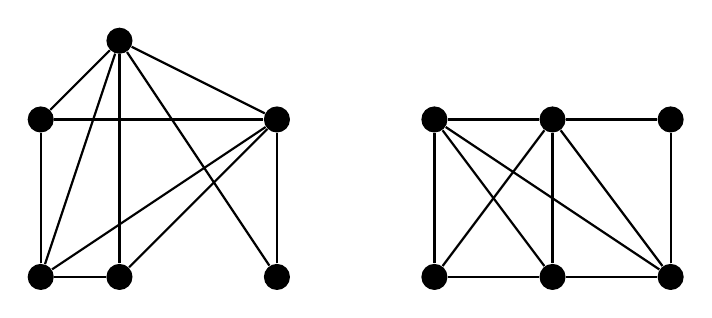
\begin{tikzpicture}
          \begin{scope}[every node/.style={circle,fill=black}]
            \node (a) at (0,0) {};
            \node (b) at (0,3) {};
            \node (c) at (2,0) {};
            \node (d) at (2,2) {};
            \node (e) at (-1,0) {};
            \node (f) at (-1,2) {};
          \end{scope}
          \begin{scope}[every edge/.style={draw=black,thick}]
            \path (a) edge (b);
            \path (a) edge (d);
            \path (a) edge (e);
            \path (b) edge (c);
            \path (b) edge (d);
              \path (b) edge (e);
              \path (b) edge (f);
              \path (c) edge (d);
              \path (d) edge (e);           
              \path (d) edge (f);
              \path (e) edge (f);
      \end{scope}
      \begin{scope}[xshift=40mm]
          \begin{scope}[every node/.style={circle,fill=black}]
            \node (a) at (0,0) {};
            \node (b) at (0,2) {};
            \node (c) at (1.5,0) {};
            \node (d) at (1.5,2) {};
            \node (e) at (3,0) {};
            \node (f) at (3,2) {};
          \end{scope}
          \begin{scope}[every edge/.style={draw=black,thick}]
            \path (a) edge (b);
            \path (a) edge (c);
            \path (c) edge (e);
            \path (a) edge (d);
            \path (b) edge (c);
            \path (b) edge (d);
              \path (b) edge (e);
              \path (b) edge (d);
              \path (d) edge (f);
              \path (c) edge (d);
              \path (d) edge (e);	            
              \path (e) edge (f);
          \end{scope}
          \end{scope}
        \end{tikzpicture}
      \end{center}
    \vspace{4mm}

\section{Strings}

\vspace{2mm}

\begin{center}
\begin{tabular}{ c|cccc } 
  & 1 & 2 & 3 & 4 \\
 \hline
 1 & 0 & 1 & 0 & 1 \\ 
 2 & 1 & 0 & 1 & 0 \\ 
 3 & 0 & 1 & 0 & 1 \\ 
 4 & 1 & 0 & 1 & 0 \\ 
\end{tabular}
\end{center}

\[0101 1010 0101 1010\]
\[s_1 = 101 10 1 \]

\vspace{2mm}

\begin{center}
\begin{tabular}{ c|cccc } 
  & 1 & 2 & 3 & 4 \\
 \hline
 1 & 0 & 0 & 1 & 1 \\ 
 2 & 0 & 0 & 1 & 1 \\ 
 3 & 1 & 1 & 0 & 0 \\ 
 4 & 1 & 1 & 0 & 0 \\ 
\end{tabular}
\end{center}

\[0011 0011 1100 1100\]
\[s_2 = 011 11 0 \]

\[A = \{0,1\} \qquad L \subseteq A^*\]

\[L = \{ s_as_b | s_a \cong s_b \} \]

\[ s_1 s_2 = 101 10 1 011 11 0 \in L \]

\end{document}
